\chapter{TỔNG QUAN ĐỀ TÀI}

\section{Giới thiệu}

Hạnh phúc của người dân là một trong những thước đo quan trọng phản ánh chất lượng cuộc sống và phát triển xã hội của mỗi quốc gia. Bên cạnh tổng sản phẩm quốc nội, các nghiên cứu về hạnh phúc còn xem xét những yếu tố như hỗ trợ xã hội, tuổi thọ khỏe mạnh, tự do trong các quyết định của cá nhân, sự hào phóng và nhận thức về tham nhũng. Những yếu tố này giúp cung cấp góc nhìn toàn diện hơn về điều kiện sống mà chỉ số kinh tế không thể phản ánh đầy đủ.

World Happiness Report là chuỗi báo cáo nghiên cứu hạnh phúc toàn cầu dựa trên dữ liệu khảo sát và các chỉ số kinh tế -- xã hội. Mỗi quốc gia được xếp hạng theo điểm hạnh phúc, đồng thời điểm số đó có thể được phân tích theo khu vực địa lý và theo nhiều năm. Tuy nhiên, dữ liệu dạng bảng có quy mô lớn và tên cột khác nhau giữa các năm có thể làm người xem khó so sánh trực tiếp. Vì vậy, đề tài \textbf{“Hệ thống trực quan hóa dữ liệu World Happiness Report”} được xây dựng nhằm chuyển dữ liệu thành các biểu đồ, bảng thống kê và công cụ tương tác dễ tiếp cận.

Nhóm sử dụng dữ liệu của giai đoạn 2015--2019, triển khai ứng dụng bằng Python và Streamlit, đồng thời sử dụng Pandas để xử lý dữ liệu và Plotly để trực quan hóa. Hệ thống không chỉ hiển thị giá trị của từng quốc gia mà còn hỗ trợ theo dõi xu hướng, so sánh khu vực, phân tích tương quan và lọc dữ liệu theo nhiều điều kiện.

\begin{figure}[H]
\centering
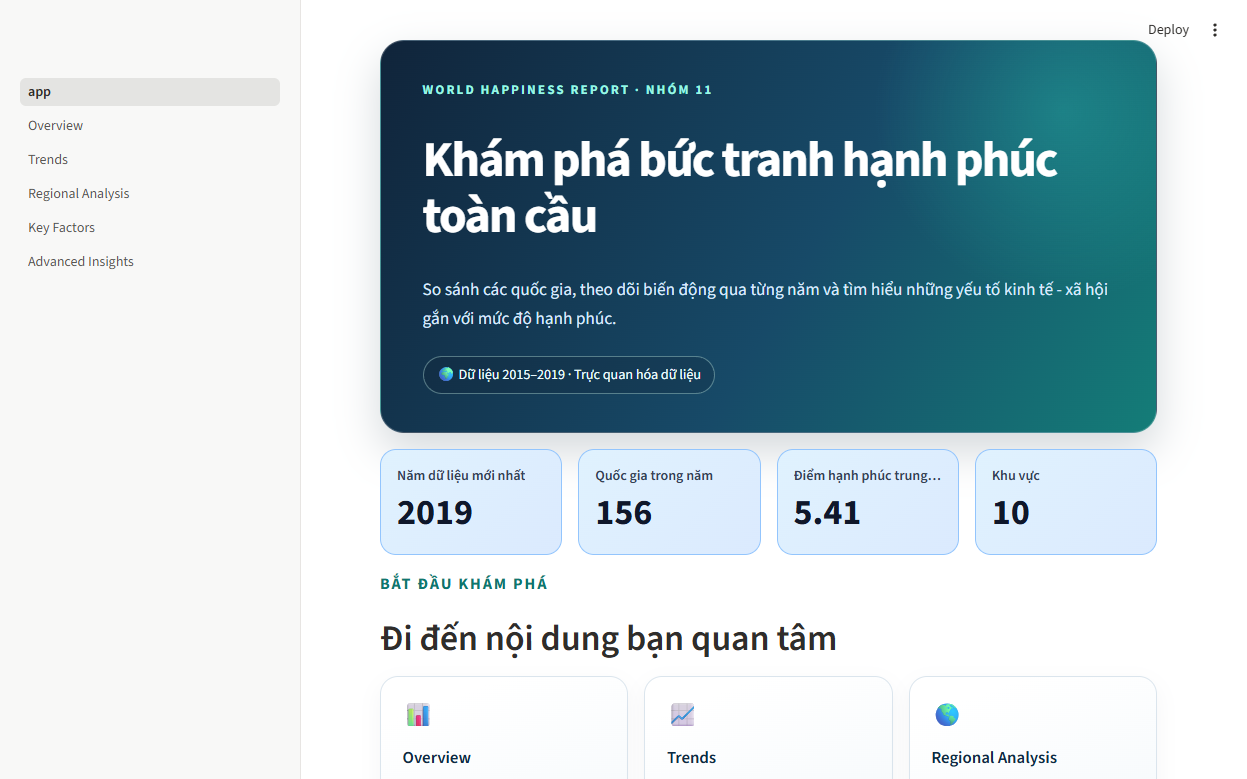
\includegraphics[width=0.92\textwidth]{images/dashboard-overview.png}
\caption{Tổng quan hệ thống trực quan hóa dữ liệu World Happiness Report}
\label{fig:tong-quan-de-tai}
\end{figure}

\section{Lý do chọn đề tài}

Dữ liệu hạnh phúc bao gồm nhiều chỉ số với thang đo, ý nghĩa và đơn vị khác nhau. Việc chỉ đọc các tệp CSV khó giúp người dùng nhanh chóng nhận ra xu hướng chung, so sánh giữa các khu vực hoặc phát hiện mối liên hệ giữa điểm hạnh phúc với GDP, tuổi thọ và các yếu tố xã hội.

Trực quan hóa dữ liệu là phương pháp phù hợp để giải quyết vấn đề này. Bản đồ, biểu đồ đường, biểu đồ cột, biểu đồ phân tán và ma trận tương quan có thể trình bày cùng một tập dữ liệu theo những góc nhìn bổ sung cho nhau. Cụ thể, đề tài đáp ứng các nhu cầu sau:

\begin{itemize}
    \item Tổ chức dữ liệu của nhiều năm theo cấu trúc thống nhất.
    \item Quan sát điểm hạnh phúc trung bình và thứ hạng của các quốc gia.
    \item So sánh mức hạnh phúc giữa các khu vực địa lý.
    \item Theo dõi biến động của điểm hạnh phúc qua thời gian.
    \item Khảo sát mối liên hệ tuyến tính giữa điểm hạnh phúc và các chỉ số kinh tế -- xã hội.
    \item Cung cấp bộ lọc để người dùng khám phá dữ liệu theo năm, khu vực, quốc gia và khoảng điểm.
\end{itemize}

\section{Mục tiêu đề tài}

\subsection{Mục tiêu chung}

Xây dựng một hệ thống dashboard trực quan, tương tác và dễ sử dụng nhằm phân tích dữ liệu World Happiness Report giai đoạn 2015--2019.

\subsection{Mục tiêu cụ thể}

\begin{itemize}
    \item Chuẩn hóa tên cột, tên quốc gia, thông tin khu vực và giá trị thiếu giữa các năm dữ liệu.
    \item Tạo trang tổng quan cho từng năm, hiển thị bảng dữ liệu và bản đồ khu vực.
    \item Xây dựng biểu đồ theo dõi xu hướng trung bình của điểm hạnh phúc, GDP và tuổi thọ khỏe mạnh.
    \item Tính hệ số tương quan Pearson giữa các cặp chỉ số quan trọng.
    \item So sánh điểm hạnh phúc theo khu vực và theo từng quốc gia qua nhiều năm.
    \item Cung cấp giao diện lọc dữ liệu nâng cao để hỗ trợ khám phá tương tác.
    \item Đưa ra nhận xét mô tả dựa trên kết quả trực quan, đồng thời tránh kết luận sai lệch quan hệ nhân quả.
\end{itemize}

\section{Đối tượng và phạm vi nghiên cứu}

\subsection{Đối tượng nghiên cứu}

Đối tượng nghiên cứu của đề tài là dữ liệu điểm hạnh phúc và các chỉ số liên quan của quốc gia, bao gồm:

\begin{itemize}
    \item Điểm hạnh phúc và thứ hạng hạnh phúc.
    \item GDP bình quân đầu người.
    \item Hỗ trợ xã hội.
    \item Tuổi thọ khỏe mạnh.
    \item Tự do lựa chọn cuộc sống.
    \item Sự hào phóng.
    \item Nhận thức về tham nhũng.
    \item Khu vực địa lý và năm báo cáo.
\end{itemize}

\subsection{Phạm vi dữ liệu}

Đề tài sử dụng năm tệp dữ liệu CSV tương ứng với các báo cáo năm 2015, 2016, 2017, 2018 và 2019. Mỗi tệp chứa thông tin theo quốc gia, trong đó điểm hạnh phúc và thứ hạng được lấy làm cơ sở để xếp hạng. Cấu trúc cột có sự khác biệt giữa các năm, ví dụ tên GDP, tuổi thọ khỏe mạnh và nhận thức về tham nhũng được đặt theo các dạng tên khác nhau. Hệ thống áp dụng ánh xạ tên cột để tạo cấu trúc chung khi phân tích.

\subsection{Phạm vi chức năng}

Dashboard gồm trang chủ và các trang phân tích chính sau:

\begin{itemize}
    \item \textbf{Overview}: chọn năm, hiển thị bản đồ trực giao và lọc dữ liệu theo khu vực.
    \item \textbf{Trends}: theo dõi trung bình theo năm, biểu đồ vùng điểm hạnh phúc và biểu đồ tương quan.
    \item \textbf{Regional Analysis}: so sánh khu vực, số lượng quốc gia, điểm trung bình và xu hướng nhiều quốc gia.
    \item \textbf{Key Factors}: tính ma trận tương quan Pearson, biểu đồ tương quan và pairplot.
    \item \textbf{Advanced Insights}: lọc theo năm, điểm số và quốc gia; so sánh nhiều quốc gia; khám phá từng yếu tố.
\end{itemize}

\section{Nhiệm vụ nghiên cứu}

Để đạt được mục tiêu, nhóm thực hiện các nhiệm vụ sau:

\begin{enumerate}
    \item Thu thập, kiểm tra và phân loại dữ liệu World Happiness Report giai đoạn 2015--2019.
    \item Tiền xử lý dữ liệu: chuẩn hóa tên cột, bổ sung khu vực, xử lý giá trị thiếu và loại trùng lặp quốc gia trong từng năm.
    \item Thiết kế cấu trúc ứng dụng gồm trang chủ, trang tổng quan, trang xu hướng, trang khu vực, trang yếu tố và trang khám phá nâng cao.
    \item Xây dựng các biểu đồ thống kê, tương tác và bộ lọc phù hợp với từng câu hỏi phân tích.
    \item Kiểm tra tính nhất quán của dữ liệu, quan sát kết quả và rút ra nhận xét mô tả.
\end{enumerate}

\section{Ý nghĩa của đề tài}

Về mặt học thuật, đề tài giúp nhóm vận dụng kiến thức về tiền xử lý dữ liệu, thống kê mô tả, tương quan và trực quan hóa trong một bài toán thực tế. Nhóm có thể quan sát dữ liệu theo nhiều chiều, đồng thời hiểu rõ tác động của cách lựa chọn năm, khu vực và loại biểu đồ đối với kết quả quan sát.

Về mặt ứng dụng, dashboard hỗ trợ người dùng không cần đọc trực tiếp tệp dữ liệu vẫn có thể khám phá thông tin. Người dùng có thể tìm quốc gia có điểm cao hoặc thấp, so sánh khu vực, theo dõi xu hướng và đánh giá mức độ liên hệ tuyến tính của các chỉ số. Các kết quả được trình bày trực quan nên phù hợp cho mục đích học tập, khảo sát và truyền đạt thông tin.

\section{Cấu trúc báo cáo}

Bài tập lớn được trình bày trong ba chương chính. Chương 1 giới thiệu đề tài, bối cảnh, mục tiêu, phạm vi và nhiệm vụ nghiên cứu. Chương 2 trình bày tổng quan dữ liệu, quy trình tiền xử lý, phương pháp phân tích, công cụ và kiến trúc hệ thống. Chương 3 trình bày kết quả trên từng trang dashboard, phân tích nhận xét thu được và đánh giá sản phẩm.
